% NeurIPS 2026 Supplementary Material
\documentclass{article}

\usepackage[preprint,nonatbib]{neurips_2026}
\usepackage[utf8]{inputenc}
\usepackage[T1]{fontenc}
\usepackage[breaklinks,colorlinks]{hyperref}
\usepackage{url}
\usepackage{amsmath}
\usepackage{amsfonts}
\usepackage{amssymb}
\usepackage{microtype}
\usepackage{graphicx}
\usepackage{placeins}
\usepackage{float}
\usepackage{booktabs}
\usepackage{multirow}
\usepackage{xcolor}
\usepackage{algorithm}

\title{Supplementary Material for\\
Depth-Conditioned Pseudo-Labels for\\
Scene-Centric Unsupervised Panoptic Segmentation}

\author{Anonymous Author(s)}

\begin{document}
\maketitle

\appendix
\renewcommand{\thefigure}{\Alph{section}.\arabic{figure}}
\renewcommand{\thetable}{\Alph{section}.\arabic{table}}
% Override default bold paragraph headings with italic (per author preference)
\makeatletter
\renewcommand{\paragraph}[1]{\par\smallskip\noindent\textit{#1}\hspace{0.5em}\ignorespaces}
\makeatother

%=========================================================================
\section{Additional Qualitative Figures}
\label{sec:supp:qualitative}
%=========================================================================

\subsection{Stage-1 Pseudo-Label Trace}
\label{sec:supp:stage1_trace}

Figure~\ref{fig:supp_real_data_flow} traces the Stage-1 data flow on real Cityscapes images, showing intermediate pseudo-label outputs together with the paired RGB/label transformations used by panoptic bootstrapping and panoptic network training.

\begin{figure}[H]
\centering
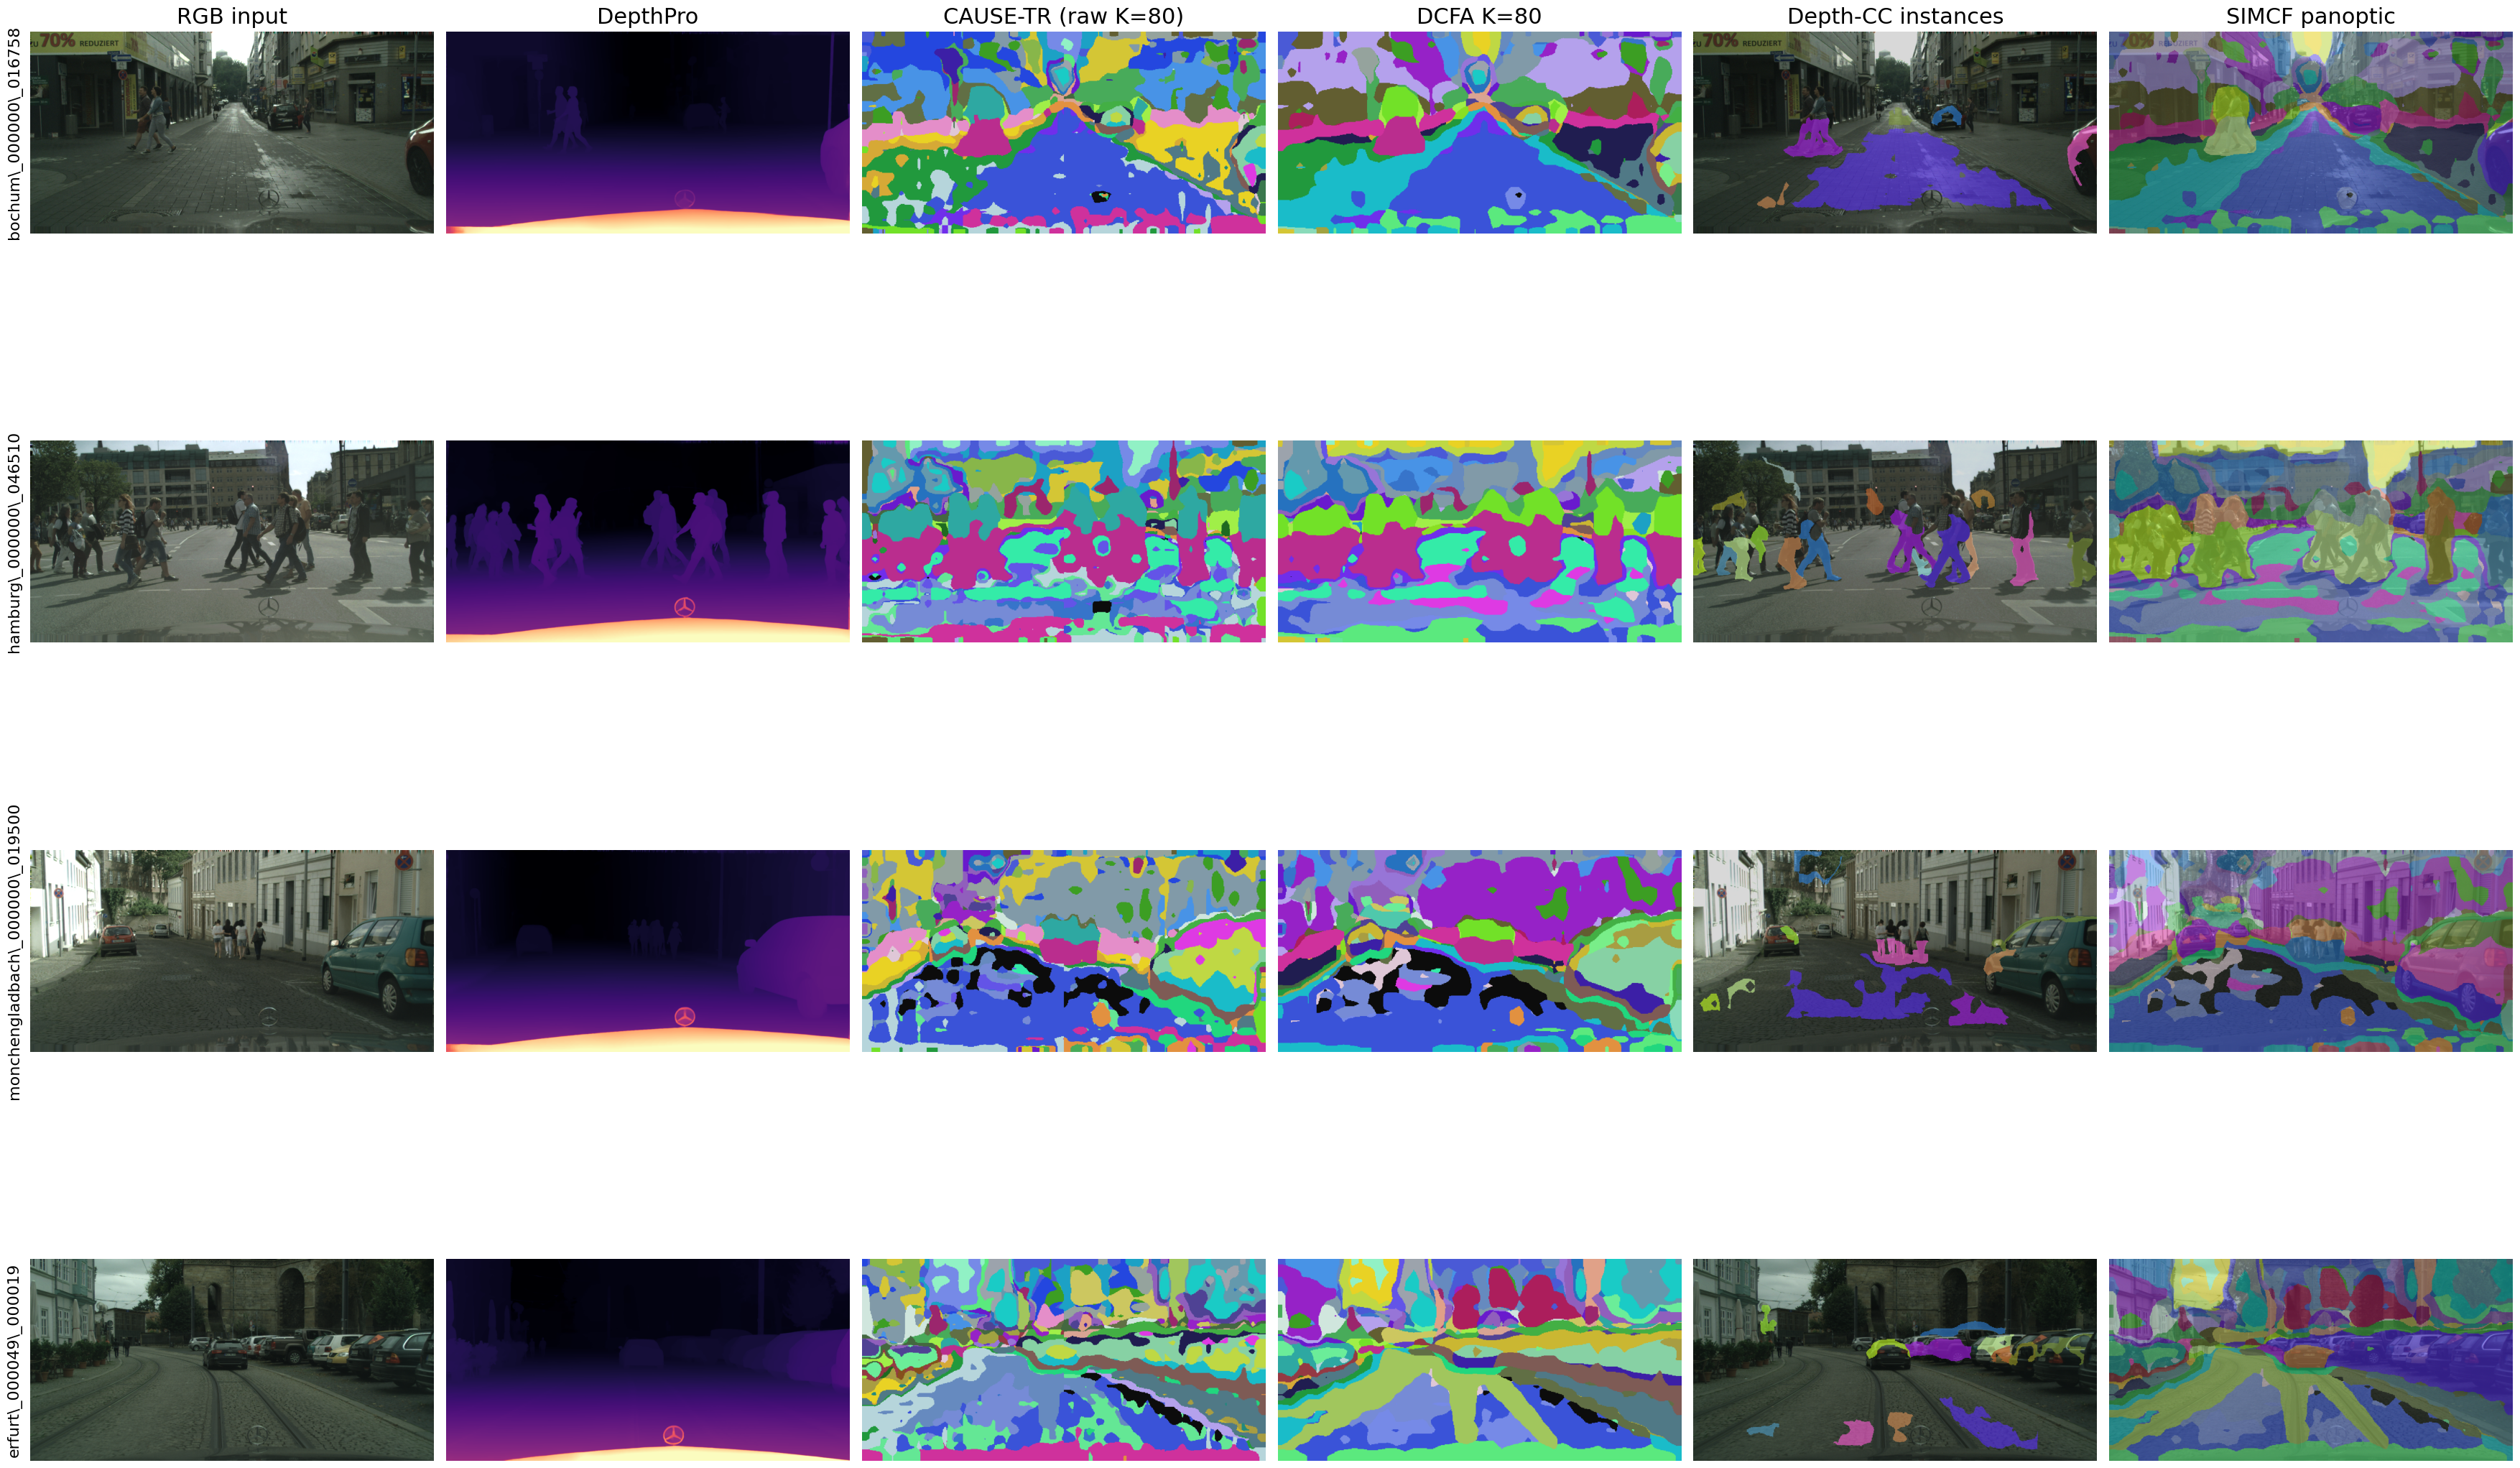
\includegraphics[width=\textwidth]{../figures/paper_ready/fig5_stage1_trace_composite.png}
\caption{Stage-1 pseudo-label trace on four Cityscapes train frames. Columns: RGB; DepthPro depth; CAUSE-TR~\cite{kim2024cause} raw $K{=}80$ clusters; DCFA-adjusted $K{=}80$; depth-CC instances on RGB; final SIMCF-filtered panoptic pseudo-labels on RGB. Row 2 (hamburg) is the canonical co-planar pedestrian failure case discussed in the main paper's Discussion and Limitations sections.}
\label{fig:supp_real_data_flow}
\end{figure}

\clearpage

\subsection{Stage-3 Panoptic Predictions}
\label{sec:supp:stage3_predictions}

Figure~\ref{fig:supp_qualitative_stage3} shows representative panoptic predictions from the trained Stage-3 network on nine Cityscapes val images, none of which were used for training. Each row presents the input RGB, the panoptic prediction colorized in the $K=80$ pseudo-class space, and the prediction overlaid on the input.

\begin{figure}[H]
\centering
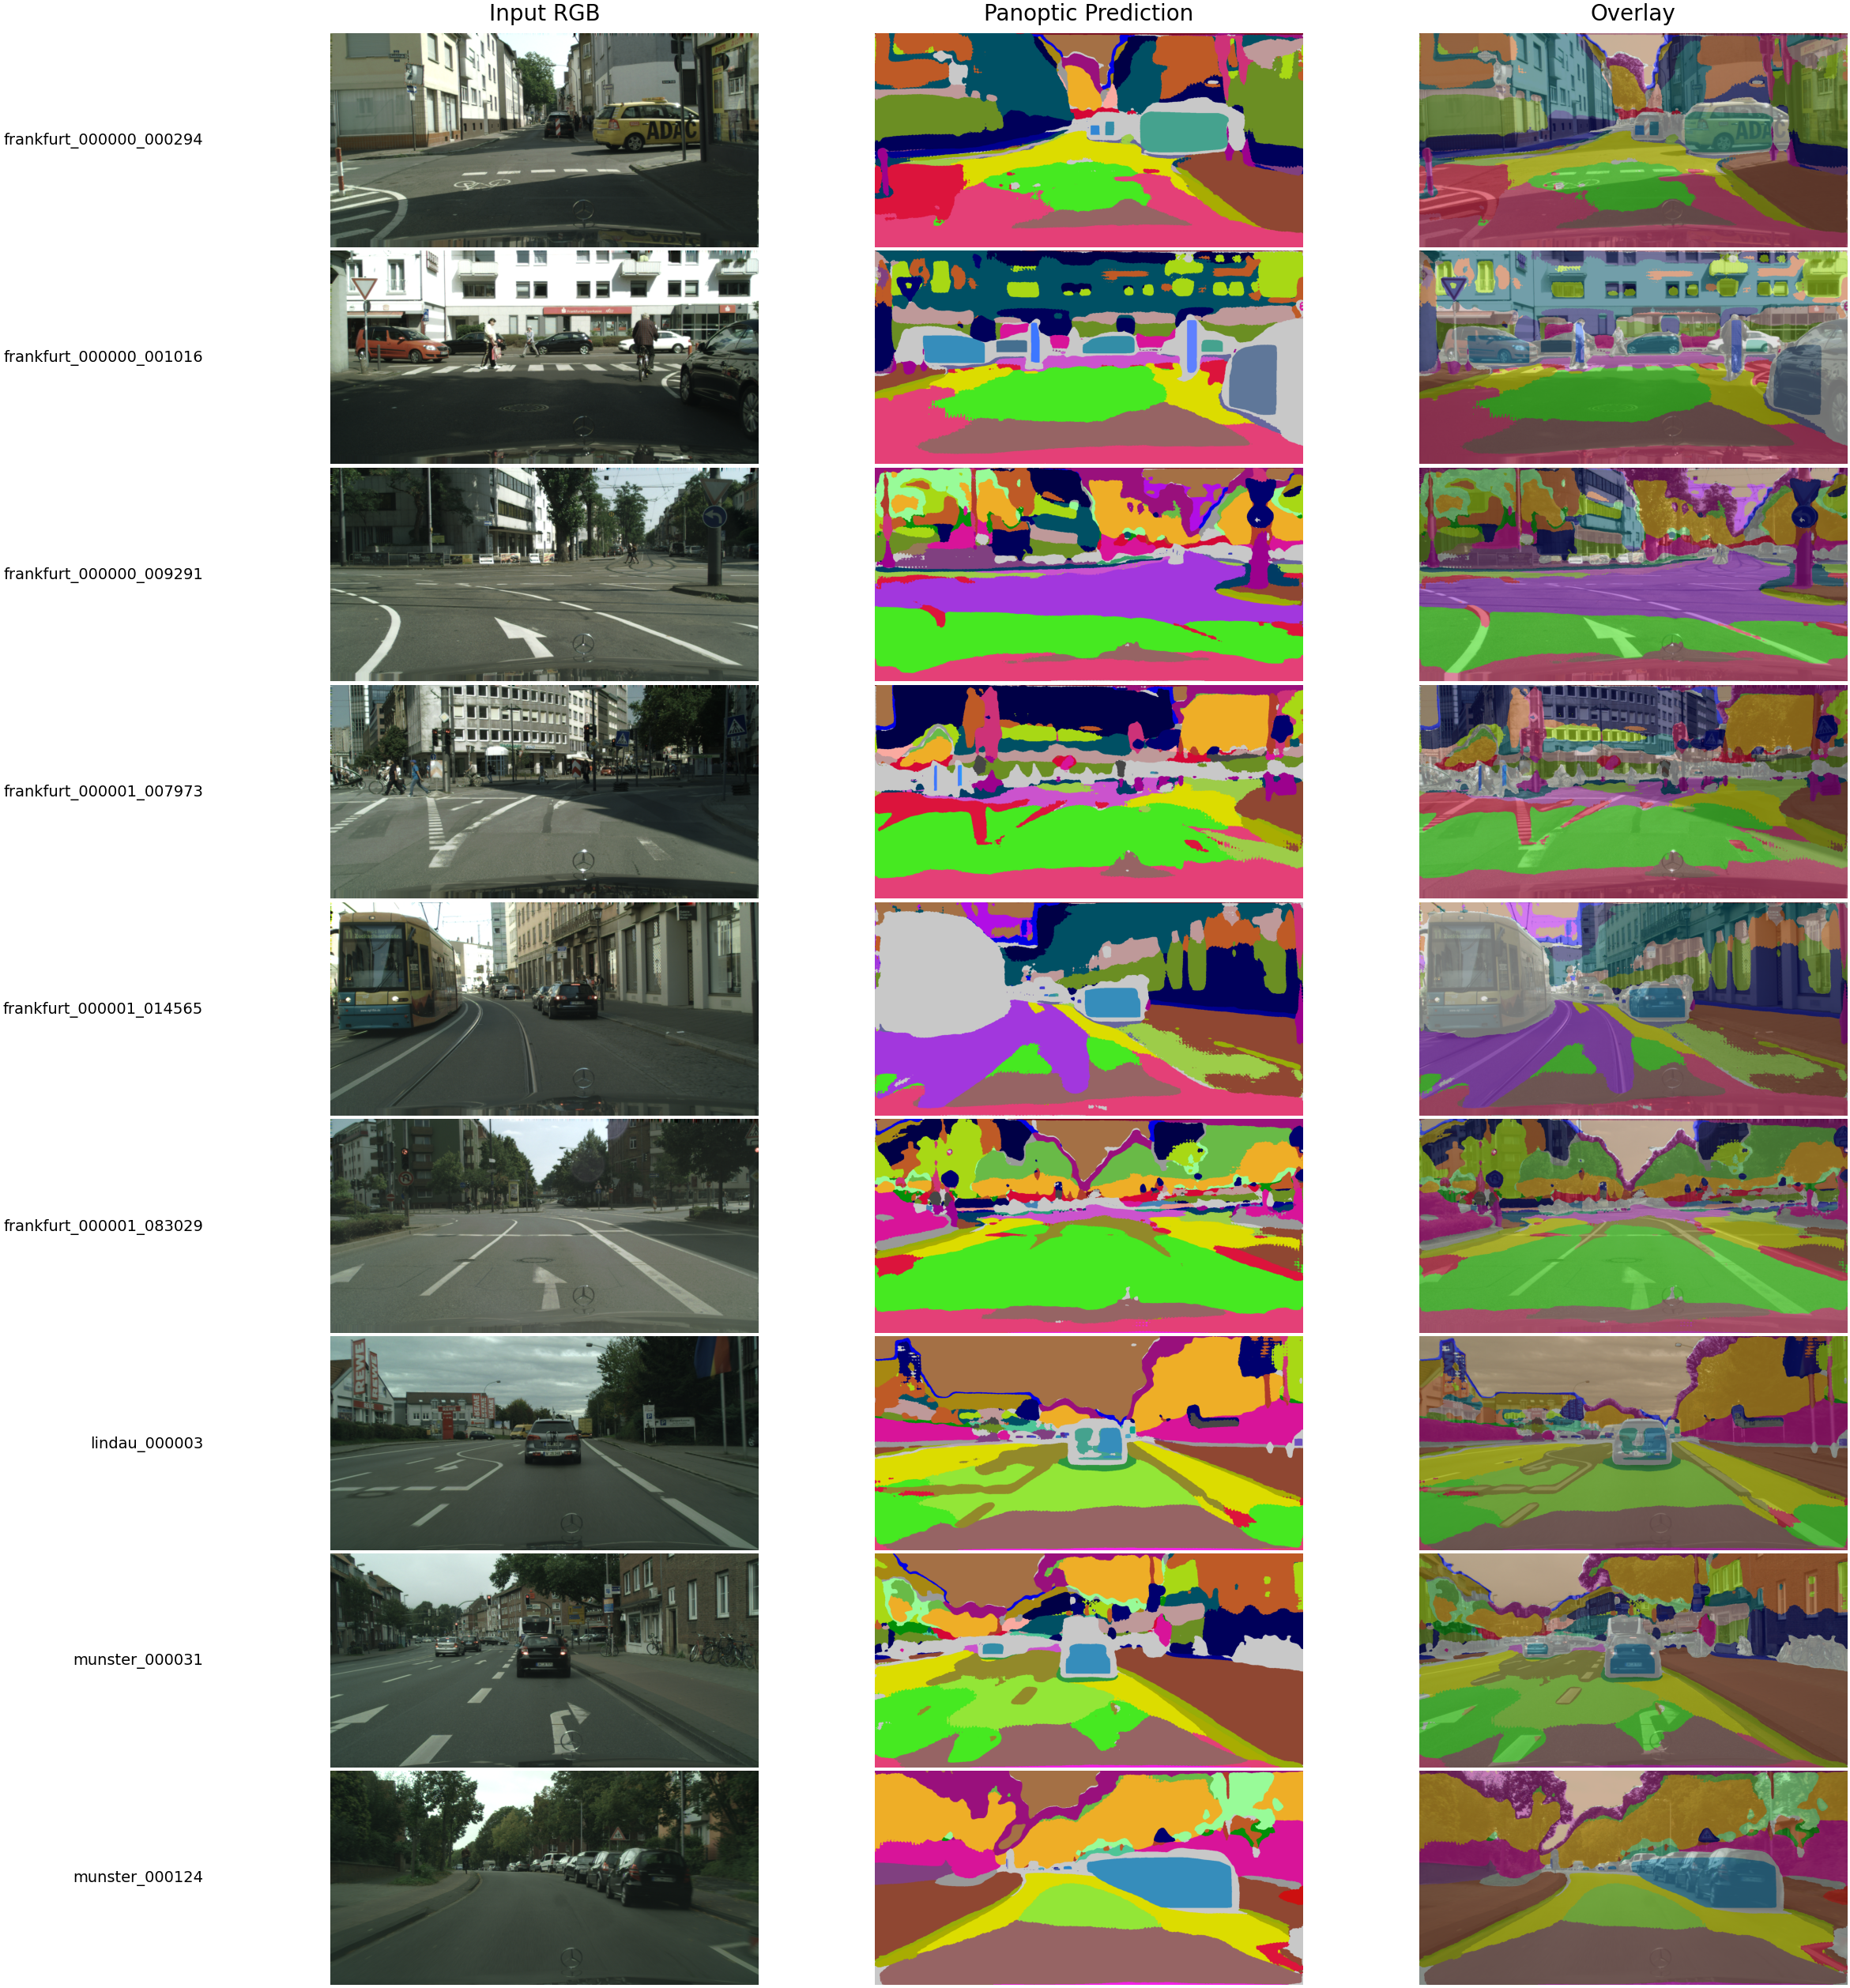
\includegraphics[width=0.92\linewidth]{../figures/paper_ready/qualitative_stage3.png}
\caption{Stage-3 panoptic predictions on Cityscapes val (9 held-out images). Columns: RGB input, panoptic prediction in the $K=80$ pseudo-class space, RGB overlay ($\alpha{=}0.55$). Hungarian alignment to the 27-class Cityscapes evaluation taxonomy is computed only at metric time and is not applied here, so colors track pseudo-class IDs rather than benchmark classes. Light grey marks pixels that the network rejects below its semantic confidence threshold (void).}
\label{fig:supp_qualitative_stage3}
\end{figure}

\clearpage

%=========================================================================
\section{Implementation Details}
\label{sec:supp:impl}
%=========================================================================

This appendix expands the abbreviated experimental setup of the main paper (Section~4.1) with the full hyperparameter, optimizer, augmentation, and hardware configuration used for every reported result. All operating hyperparameters were fixed before consulting Cityscapes annotations and were not retuned afterwards.

\subsection{Datasets and Evaluation Protocol}
\label{sec:supp:impl:data}

Pseudo-label generation and panoptic network training use only Cityscapes train~\cite{cordts2016cityscapes} (2{,}975 images, no annotations). Evaluation is on Cityscapes val (500 images) under the 27-class CAUSE~\cite{kim2024cause} pseudo-vocabulary with a Hungarian map to the 27-class Cityscapes label space (\texttt{NUM\_CLASSES=27} in the official CUPS protocol~\cite{hahn2025cups}). The 27-class evaluation taxonomy includes the 19 standard semantic-segmentation classes plus parking, rail track, guard rail, bridge, tunnel, polegroup, caravan, and trailer. Cross-dataset transfer follows the CUPS~\cite{hahn2025cups} protocol on KITTI~\cite{geiger2012kitti}, Waymo V2~\cite{sun2020waymo}, and Mapillary Vistas v2.

\subsection{Stage-1: Pseudo-Label Generation}
\label{sec:supp:impl:stage1}

\paragraph{Frozen priors.}
DINOv2 ViT-B/14~\cite{oquab2024dinov2} backbone (no fine-tuning) and CAUSE-TR head~\cite{kim2024cause} (frozen, 90-dimensional concept-clusterbook code).

\paragraph{DCFA training.}
Hidden width $h{=}384$, two-layer MLP, 16-dimensional sinusoidal depth positional embedding, $\sim$40K trainable parameters. Loss: depth-correlation term $+\,\lambda_p \mathcal{L}_\text{preserve}$ with $\lambda_p{=}20$. Optimizer: AdamW, learning rate $10^{-3}$, weight decay $10^{-4}$, 10K iterations, batch size 32 images, sampling 1024 pixels and 1024 pixel pairs per image. The preservation term anchors the residual update to identity at initialisation and is re-applied at every step. Wall-clock: $\approx 1$ hour on a single GTX 1080 Ti.

\paragraph{$k$-means over-clustering.}
$k{=}80$ centroids on L2-normalised DCFA-adjusted CAUSE-TR codes, fitted on the 2{,}975 Cityscapes train images using \texttt{scikit-learn} mini-batch $k$-means (batch 4096, 100 iterations, fixed random seed). Centroids are saved once and reused throughout the rest of the pipeline.

\paragraph{Instance branch.}
DepthPro~\cite{bochkovskii2024depthpro} monocular depth (frozen, no fine-tuning). $3\times3$ Sobel kernels, gradient threshold $\tau_d{=}0.20$, 8-neighbour connected components inside thing-eligible semantic regions, $A_\text{min}{=}1000$ pixel filter, three iterations of $3\times3$ dilation.

\paragraph{SIMCF.}
Feature similarity threshold $\tau_\text{sim}{=}0.85$, depth-implausibility multiplier $\eta{=}2.5$. Adjacent-proposal merging (Step~B) and depth-implausibility void rejection (Step~C) are applied in this order.

\subsection{Stage-2: Panoptic Bootstrapping}
\label{sec:supp:impl:stage2}

Cascade Mask R-CNN~\cite{cai2018cascade} with three cascade stages on a frozen DINOv3 ViT-B/16 backbone~\cite{simeoni2025dinov3} (no backbone fine-tuning). 8K optimizer steps, batch size 8 (4 per GPU), AdamW (lr $10^{-4}$, weight decay $0.05$, $\beta_1{=}0.9$, $\beta_2{=}0.999$), cosine schedule with 500-step linear warmup. Loss includes DropLoss~\cite{wang2023cutler} ($\lambda_\text{drop}{=}1.0$) and self-enhanced copy-paste augmentation. Augmentation: random horizontal flip, random scale jitter $[0.5, 2.0]$, random crop $1024\times1024$, copy-paste with probability 0.5, photometric jitter (brightness $\pm$0.2, contrast $\pm$0.2, saturation $\pm$0.2). Wall-clock: $\approx 12$ hours on $2\times$ NVIDIA GTX 1080 Ti with PyTorch DistributedDataParallel.

\subsection{Stage-3: EMA Self-Training}
\label{sec:supp:impl:stage3}

Three EMA self-training rounds, each 5K optimizer steps. EMA coefficient 0.999. Three-scale teacher (scales $\{0.75, 1.0, 1.25\}$) with class-aware confidence thresholding (foreground $0.4$, background $0.3$). Same augmentation pipeline as Stage-2; same optimizer family and learning-rate base ($5\times10^{-5}$ at the start of each round, cosine schedule per round). Wall-clock: $\approx 16$ hours total on $2\times$ GTX 1080 Ti.

\subsection{Hardware and Wall-Clock Budget}
\label{sec:supp:impl:hardware}

All training is performed on $2\times$ NVIDIA GTX 1080 Ti GPUs (consumer-grade, 11 GB VRAM each) with PyTorch DistributedDataParallel. Total compute footprint per pipeline run: Stage-1 generation $\approx 2$ GPU-hours, Stage-2 bootstrapping $\approx 24$ GPU-hours ($\approx 12$ wall-clock on 2 GPUs), Stage-3 self-training $\approx 32$ GPU-hours ($\approx 16$ wall-clock on 2 GPUs); aggregate $\approx 58$ GPU-hours. The pipeline is therefore feasible on consumer-grade hardware that lacks the calibrated stereo rigs and synchronized video required by CUPS~\cite{hahn2025cups} at pseudo-label time.

\subsection{SIMCF Pseudocode}
\label{sec:supp:impl:simcf_alg}

\begin{algorithm}[H]
\caption{SIMCF$(S_x^0,I_x^0,D,\phi,v;\tau_\text{sim},\eta)$. $\phi$ maps over-clusters to the 27-class CAUSE taxonomy; $v$ is dense DINOv3 features.}
\label{alg:simcf}
\begin{enumerate}
\setlength{\itemsep}{0pt}
\item $(\hat S_x,\hat I_x) \gets (S_x^0,I_x^0)$
\item \textit{for each} instance region $R_k=\{p:\hat I_x(p)=k\}$ \textit{do}
\item \quad $c_k \gets \arg\max_c |\{p\in R_k:\phi(\hat S_x(p))=c\}|$
\item \quad $s_k \gets \arg\max_s |\{p\in R_k:\hat S_x(p)=s,\ \phi(s)=c_k\}|$
\item \quad \textit{for each} $p\in R_k$ with $\phi(\hat S_x(p))\ne c_k$ \textit{do} $\hat S_x(p)\gets s_k$
\item \textit{for each} adjacent proposal pair $(a,b)$ in $\hat I_x$ \textit{do}
\item \quad compute mean features $\bar v_a,\bar v_b$ over $R_a,R_b$
\item \quad \textit{if} $c_a=c_b$ and $\cos(\bar v_a,\bar v_b)>\tau_\text{sim}$ \textit{then} merge $R_a$ and $R_b$ in $\hat I_x$
\item \textit{for each} pseudo-class $c$ \textit{do}
\item \quad $P_c\gets\{p:\phi(\hat S_x(p))=c\}$;\quad $(\mu_c,\sigma_c)\gets(\operatorname{mean}D(P_c),\operatorname{std}D(P_c))$
\item \textit{for each} pixel $p$ \textit{do}
\item \quad $c\gets\phi(\hat S_x(p))$
\item \quad \textit{if} $|D(p)-\mu_c|>\eta\sigma_c$ \textit{then} $\hat S_x(p)\gets\mathrm{void}$; $\hat I_x(p)\gets0$
\item \textit{return} $(\hat S_x,\hat I_x)$
\end{enumerate}
\end{algorithm}

\subsection{DCFA Loss Definitions}
\label{sec:supp:impl:dcfa_loss}

Let $\mathcal{U}$ denote the set of $|\mathcal{U}| = 1024$ pixels sampled per image and $\mathcal{P}$ the set of $|\mathcal{P}| = 1024$ pixel pairs sampled from $\mathcal{U}$. Then
\begin{align*}
\mathcal{L}_\text{corr} &= \tfrac{1}{|\mathcal{P}|}\!\!\sum_{(i,j)\in\mathcal{P}} \mathcal{K}_{\sigma_d}(D_i, D_j)\,\big(1 - \cos(\tilde z_i, \tilde z_j)\big), \\
\mathcal{L}_\text{preserve} &= \tfrac{1}{|\mathcal{U}|} \sum_{u \in \mathcal{U}} \|\tilde z_u - z_u\|_2^2,
\end{align*}
where $\mathcal{K}_{\sigma_d}$ is the DepthG~\cite{sick2024depthg} depth-similarity kernel with bandwidth $\sigma_d=0.5$. Both losses are averaged over the sampled set per image, then averaged over the minibatch.

\subsection{Reproducibility Notes}
\label{sec:supp:impl:repro}

All random seeds are fixed at the beginning of each stage (DCFA training seed $42$, $k$-means seed $0$, Stage-2/3 dataloader seed $42$). Implementation: Python 3.10, PyTorch 2.1, Detectron2 0.6, CUDA 11.8. Stage-1 pseudo-labels and Stage-2/3 checkpoints will be released alongside the code upon publication.

%=========================================================================
\section{SIMCF Threshold Sensitivity}
\label{sec:supp:simcf_sweep}
%=========================================================================

SIMCF exposes two thresholds: $\tau_\text{sim}$ for adjacent-proposal feature merging (Step~B) and $\eta$ for depth-implausibility void rejection (Step~C). To verify that SIMCF's contribution is not the product of threshold tuning, we sweep both $\pm{\sim}12\%$ around the paper setting and re-evaluate pseudo-label quality on the full Cityscapes train set ($N{=}2975$).

\begin{table}[H]
\caption{SIMCF threshold sensitivity at fixed depth instances ($\tau_d{=}0.20$, DepthPro). Pseudo-label PQ is computed on Cityscapes train under the CUPS~\cite{hahn2025cups} 27-class protocol.}
\label{tab:simcf_sensitivity}
\centering
\small
\setlength{\tabcolsep}{6pt}
\begin{tabular}{l c c c c c c}
\toprule
Setting & $\tau_\text{sim}$ & $\eta$ & PQ & SQ & RQ & mIoU \\
\midrule
tighter         & 0.75 & 2.0 & 25.98 & 58.79 & 34.55 & 56.08 \\
baseline (paper) & 0.85 & 2.5 & 25.87 & 58.38 & 34.83 & 56.17 \\
looser          & 0.95 & 3.0 & 25.27 & 57.63 & 34.10 & 56.22 \\
\bottomrule
\end{tabular}
\end{table}

\paragraph{Interpretation.}
Pseudo-label PQ varies within a 0.71-point band (25.27--25.98) across the sweep, smaller than the $+1.31$ PQ super-additive gap from either single component to Both reported in the main paper's Table~3. Tighter thresholds slightly improve PQ (more aggressive merging recovers more depth over-fragmentations); looser thresholds degrade modestly. The mechanism is therefore robust to moderate threshold perturbation rather than tuned-on-test.

%=========================================================================
\section{Depth Model Ablation}
\label{sec:supp:depth}
%=========================================================================

We compared three monocular depth estimators (SPIdepth, Depth-Anything v3~\cite{lin2025da3}, DepthPro~\cite{bochkovskii2024depthpro}) under representative gradient thresholds at the Stage-1 pseudo-label level. The rows in Table~\ref{tab:depth} are not a single leaderboard: some use the raw $K{=}80$ semantic map and others use the DCFA semantic map. They are reported jointly to separate mask quality from recognition quality while choosing the training-data configuration.

\begin{table}[H]
\caption{Depth and threshold diagnostics with aggregate SQ/RQ on Cityscapes train pseudo-labels.}
\label{tab:depth}
\centering
\small
\setlength{\tabcolsep}{6pt}
\begin{tabular}{l l c c c c}
\toprule
Depth & Sem. & $\tau$ & PQ & SQ & RQ \\
\midrule
SPIdepth & raw $K$=80 & 0.20 & 26.74 & 71.88 & 31.41 \\
DA v3~\cite{lin2025da3} & raw $K$=80 & 0.03 & 27.37 & 73.44 & 35.66 \\
DA v3~\cite{lin2025da3} & DCFA & 0.20 & 26.44 & 61.37 & 35.83 \\
DepthPro~\cite{bochkovskii2024depthpro} & DCFA & 0.01 & 27.81 & 63.07 & 37.40 \\
DepthPro~\cite{bochkovskii2024depthpro} & DCFA & 0.20 & 26.13 & 60.63 & 35.80 \\
\bottomrule
\end{tabular}
\end{table}

\paragraph{Discussion.}
The table shows why PQ alone is not a sufficient diagnostic for the depth branch. The sharper $\tau{=}0.01$ DepthPro setting has stronger standalone PQ/SQ/RQ, but it produces a fragmented training set with roughly 57 instances per image and more than half below 1000 pixels. The $\tau{=}0.20$ setting has lower standalone PQ but produces larger training targets, roughly 22 instances per image, which is the configuration used for panoptic bootstrapping. DA v3 at the same training-data threshold reaches a similar RQ, indicating that the choice is governed by the training signal produced by the depth branch rather than by the stuff/thing aggregate split.

%=========================================================================
\section{Out-of-Distribution Sanity Checks}
\label{sec:supp:ood}
%=========================================================================

The main paper reports cross-dataset transfer on three driving-scene benchmarks (KITTI, Waymo V2, Mapillary v2 in Section~4.3) where the Cityscapes-derived pseudo-label vocabulary is in-domain. We additionally run two out-of-distribution sanity checks: (i) MOTS~\cite{voigtlaender2019mots} as a thing-only label space whose vocabulary is a subset of Cityscapes-things, and (ii) COCO-Stuff-27~\cite{caesar2018coco} as a vocabulary-mismatched object-centric dataset whose 27 classes overlap only partially with Cityscapes-27. Table~\ref{tab:cocooo} reports the result.

\begin{table}[H]
\caption{Out-of-distribution sanity checks on a thing-only label space (MOTS) and a vocabulary-mismatched object-centric dataset (COCO-Stuff-27). All numbers are percentages.}
\label{tab:cocooo}
\centering
\footnotesize
\setlength{\tabcolsep}{6pt}
\begin{tabular}{l c c c c}
\toprule
Dataset (OOD) & \# img & PQ & SQ & RQ \\
\midrule
MOTS~\cite{voigtlaender2019mots} thing-only & 2{,}862 & 61.10 & 88.71 & 65.80 \\
\quad CUPS~\cite{hahn2025cups} ref. & --- & 86.4 & 86.4 & 76.9 \\
COCO-Stuff-27~\cite{caesar2018coco} vocab.\ mismatch & 1{,}000 & \phantom{0}7.83 & 38.55 & 10.06 \\
\bottomrule
\end{tabular}
\end{table}

\paragraph{Interpretation.}
The MOTS result (61.10 PQ, SQ 88.71) confirms that mask geometry generalizes to a thing-only OOD vocabulary: the Stage-3 network produces high-quality masks on KITTI-style sequences even when the label space drops from 27 classes to a thing-only subset. The gap to the CUPS~\cite{hahn2025cups} reference (86.4 PQ) is recognition-driven (RQ 65.80 vs.\ 76.9) and reflects vocabulary granularity rather than a transfer failure of the architecture. The COCO-Stuff-27 result (7.83 PQ) is dominated by categories absent from a Cityscapes-derived pseudo-label space: most COCO-Stuff-27 categories (e.g.\ kitchenware, sports gear, food) have no analog in the Cityscapes pseudo-vocabulary and are unrecoverable by Hungarian alignment alone. This is the vocabulary boundary of in-domain training and not a transfer failure of the architecture; resolving it would require expanding the pseudo-label generator's vocabulary at training time, which is orthogonal to the contributions of this paper.

%=========================================================================
\section{Per-Class Cityscapes Metrics}
\label{sec:supp:perclass}
%=========================================================================

Table~\ref{tab:perclass} reports per-class PQ/SQ/RQ for the final trained network of the main paper (35.83 PQ aggregate, Section~4.2) under the CUPS~\cite{hahn2025cups} 27-class evaluation protocol with Hungarian matching from the $K{=}80$ pseudo-vocabulary to the 27-class Cityscapes label space.

\begin{table}[H]
\caption{Per-class Cityscapes validation metrics for the final trained network. Values are percentages. Six classes (parking, guard rail, tunnel, polegroup, caravan, trailer) are vocabulary-dead; the twenty active classes carry the 35.83 PQ aggregate reported in the main paper.}
\label{tab:perclass}
\centering
\small
\setlength{\tabcolsep}{6pt}
\resizebox{\textwidth}{!}{%
\begin{tabular}{l c c c l c c c l c c c}
\toprule
Class & PQ & SQ & RQ & Class & PQ & SQ & RQ & Class & PQ & SQ & RQ \\
\midrule
road & 93.0 & 95.0 & 97.9 & tunnel & 0.0 & 0.0 & 0.0 & rider & 22.9 & 62.6 & 36.6 \\
sidewalk & 62.4 & 78.5 & 79.5 & pole & 2.0 & 72.3 & 2.8 & car & 70.7 & 88.7 & 79.7 \\
parking & 0.0 & 0.0 & 0.0 & polegroup & 0.0 & 0.0 & 0.0 & truck & 62.6 & 83.8 & 74.7 \\
rail track & 8.4 & 67.2 & 12.5 & traffic light & 6.2 & 60.3 & 10.3 & bus & 76.7 & 90.8 & 84.4 \\
building & 83.5 & 85.7 & 97.5 & traffic sign & 37.2 & 65.9 & 56.4 & caravan & 0.0 & 0.0 & 0.0 \\
wall & 32.3 & 67.7 & 47.8 & vegetation & 84.7 & 85.7 & 98.8 & trailer & 0.0 & 0.0 & 0.0 \\
fence & 20.3 & 63.0 & 32.1 & terrain & 35.7 & 73.4 & 48.6 & train & 77.2 & 88.7 & 87.0 \\
guard rail & 0.0 & 0.0 & 0.0 & sky & 86.1 & 89.9 & 95.7 & motorcycle & 0.1 & 100.0 & 0.1 \\
bridge & 17.2 & 64.5 & 26.7 & person & 13.4 & 71.4 & 18.7 & bicycle & 39.0 & 77.2 & 50.5 \\
\bottomrule
\end{tabular}
}
\end{table}

\paragraph{Discussion.}
Twenty active classes carry the 35.83 PQ aggregate. Large stuff regions (road 93.0, sky 86.1, vegetation 84.7, building 83.5) and large vehicles (car 70.7, bus 76.7, train 77.2) score above 70 PQ, since frozen semantic codes produce coherent regions and depth boundaries align with object extent. The remaining seven classes are vocabulary-coverage cases: parking, guard rail, tunnel, polegroup, caravan, and trailer lie outside the standard Cityscapes-19 panoptic benchmark and receive few positive examples in the $K{=}80$ over-cluster vocabulary, while motorcycle matches a single near-perfect instance (SQ$=$100). These cases reflect a property of the pseudo-label vocabulary rather than the network architecture, and their effect on the aggregate is bounded: removing them and averaging only over the standard Cityscapes-19 panoptic classes raises the protocol comparability of our headline.

The per-class table also exposes the recognition bottleneck for closely-spaced object classes: person reaches SQ$=$71.4 and rider SQ$=$62.6 (both above the 60-point band that classifies the per-class match as geometrically correct), while their RQ values (18.7 and 36.6 respectively) are recognition-limited by depth-based instance separation on co-planar pedestrian crowds. This is the failure mode discussed in the main paper's Conclusion (Section~5).

\paragraph{SIMCF feature-merge diagnostics.}
Two qualitative metrics from the feature-guided merge step (Step~B) of SIMCF complete the picture. Average pseudo-instance count per image drops from 44 before the merge to 22 after, median instance size grows from 5{,}502 to 14{,}965 pixels, and stuff contamination falls from 50.7\% to 28.0\%. Many depth gradients are intra-object surface changes rather than object boundaries, and merging fragments whose semantic identity and dense appearance agree recovers the single-object structure that monocular depth had over-fragmented.

%=========================================================================
\section{Broader Impact}
\label{sec:impact}
%=========================================================================

\noindent Removing stereo and motion requirements at pseudo-label time broadens the range of imagery to which scene-centric unsupervised panoptic segmentation can be applied. The intended beneficiaries are autonomous-driving and robotic-perception pipelines that ingest monocular footage from phones, dashcams, or fixed cameras, where calibrated stereo rigs and synchronized video are unavailable.

The same property creates dual-use risk. A monocular-only pipeline lowers the data and hardware bar for deployment in surveillance and behavioral-monitoring settings that the original stereo-based methods could not easily reach. We do not release pretrained weights tuned to specific surveillance contexts, and the system as evaluated targets street-scene categories rather than person re-identification.

Two technical-bias concerns also follow from the design. First, the frozen pseudo-label vocabulary inherits any class-imbalance and dataset-bias signal already present in CAUSE-TR's~\cite{kim2024cause} Cityscapes-derived clusterbook; six dead classes, discussed in the main paper's limitations section, are a direct symptom and would compound on demographically less-represented scenes. Second, depth-based instance separation degrades on co-planar pedestrian crowds, which are over-represented in dense urban settings and may correlate with population density or geography. These limitations should be accounted for before downstream deployment, particularly in settings where the consequences of mispredicted person-class instances are non-trivial.

%=========================================================================
\begin{thebibliography}{99}
%=========================================================================
\bibitem{cordts2016cityscapes} M.~Cordts, M.~Omran, S.~Ramos, et~al. The Cityscapes dataset for semantic urban scene understanding. \emph{CVPR}, 2016.
\bibitem{voigtlaender2019mots} P.~Voigtlaender, M.~Krause, A.~Osep, et~al. MOTS: Multi-object tracking and segmentation. \emph{CVPR}, 2019.
\bibitem{geiger2012kitti} A.~Geiger, P.~Lenz, R.~Urtasun. Are we ready for autonomous driving? The KITTI vision benchmark suite. \emph{CVPR}, 2012.
\bibitem{sun2020waymo} P.~Sun, H.~Kretzschmar, X.~Dotiwalla, et~al. Scalability in perception for autonomous driving: Waymo Open Dataset. \emph{CVPR}, 2020.
\bibitem{caesar2018coco} H.~Caesar, J.~Uijlings, V.~Ferrari. COCO-Stuff: Thing and stuff classes in context. \emph{CVPR}, 2018.
\bibitem{oquab2024dinov2} M.~Oquab, T.~Darcet, T.~Moutakanni, et~al. DINOv2: Learning robust visual features without supervision. \emph{TMLR}, 2024.
\bibitem{simeoni2025dinov3} O.~Sim\'eoni, et~al. DINOv3. \emph{arXiv preprint arXiv:2508.10104}, 2025.
\bibitem{kim2024cause} J.~Kim, et~al. Causal unsupervised semantic segmentation. \emph{arXiv preprint arXiv:2310.07379}, 2024.
\bibitem{bochkovskii2024depthpro} A.~Bochkovskii, et~al. Depth Pro: Sharp monocular metric depth in less than a second. \emph{arXiv preprint arXiv:2410.02073}, 2024.
\bibitem{lin2025da3} D.~Lin, et~al. Depth Anything 3: Recovering the visual space from any views. \emph{arXiv preprint arXiv:2511.10647}, 2025.
\bibitem{cai2018cascade} Z.~Cai, N.~Vasconcelos. Cascade R-CNN: Delving into high quality object detection. \emph{CVPR}, 2018.
\bibitem{wang2023cutler} X.~Wang, et~al. Cut and Learn for unsupervised object detection and instance segmentation. \emph{CVPR}, 2023.
\bibitem{hahn2025cups} A.~Hahn, et~al. Scene-centric unsupervised panoptic segmentation (CUPS). \emph{CVPR}, 2025.
\bibitem{sick2024depthg} N.~Sick, et~al. Unsupervised semantic segmentation through depth-guided feature correlation and sampling. \emph{CVPR}, 2024.
\end{thebibliography}

\end{document}
